\chapter{Related Work}\label{ch:related_work}

\lettrine[lines=4, loversize=-0.1, lraise=0.1]{A}{ccording} to \citet{yauch}, it is very difficult to measure agility, although it has been widely spread. \citet{tsourveloudis} agree on this mainly because of the vagueness of agility's concept. Nevertheless, various tools have been developed in the last decade in order to measure the agility in software development teams. Below is a short description of some that have been used as references in many papers in this field. The tools are separated into two categories, 
\begin{inparaenum} [a\upshape)]
\item those which measure how agile really are the agile methodologies
\item those which measure the agility of software development teams.
\end{inparaenum}

\section{How agile are the agile methodologies}

\subsection{Balancing Discipline and Agility}
\citet{1231450} did not come up with a tool to measure agility but rather to balance between agility and discipline. According to them, discipline is the foundation for any successful endeavour and creates experience, history and well-organized memories. On the other hand, agility is described as a counterpart of discipline. Agility uses the memory and history in order to adjust to the context in which it is applied and takes advantage of the unexpected opportunities that might come up. The combination of the two can bring success to an organisation. In their research, \citet{1231450}, came up with five ``critical decision factors" which can determine if an agile or plan-driven method is suitable for a software development project.

Figure~\ref{fig:boehm_turner_5axes} depicts these factors:
\begin{inparaenum} [a\upshape)]
\item size of a team working in a project
\item criticality of damage of unexpected defects
\item culture needed to balance between chaos and order
\item dynamism of the team working in chaos or in a planned way
\item personnel which refers to the extended \citet{cockburn2002agile} skill rating %search more
\end{inparaenum}

\begin{figure}[H]
\ffigbox[\FBwidth] {
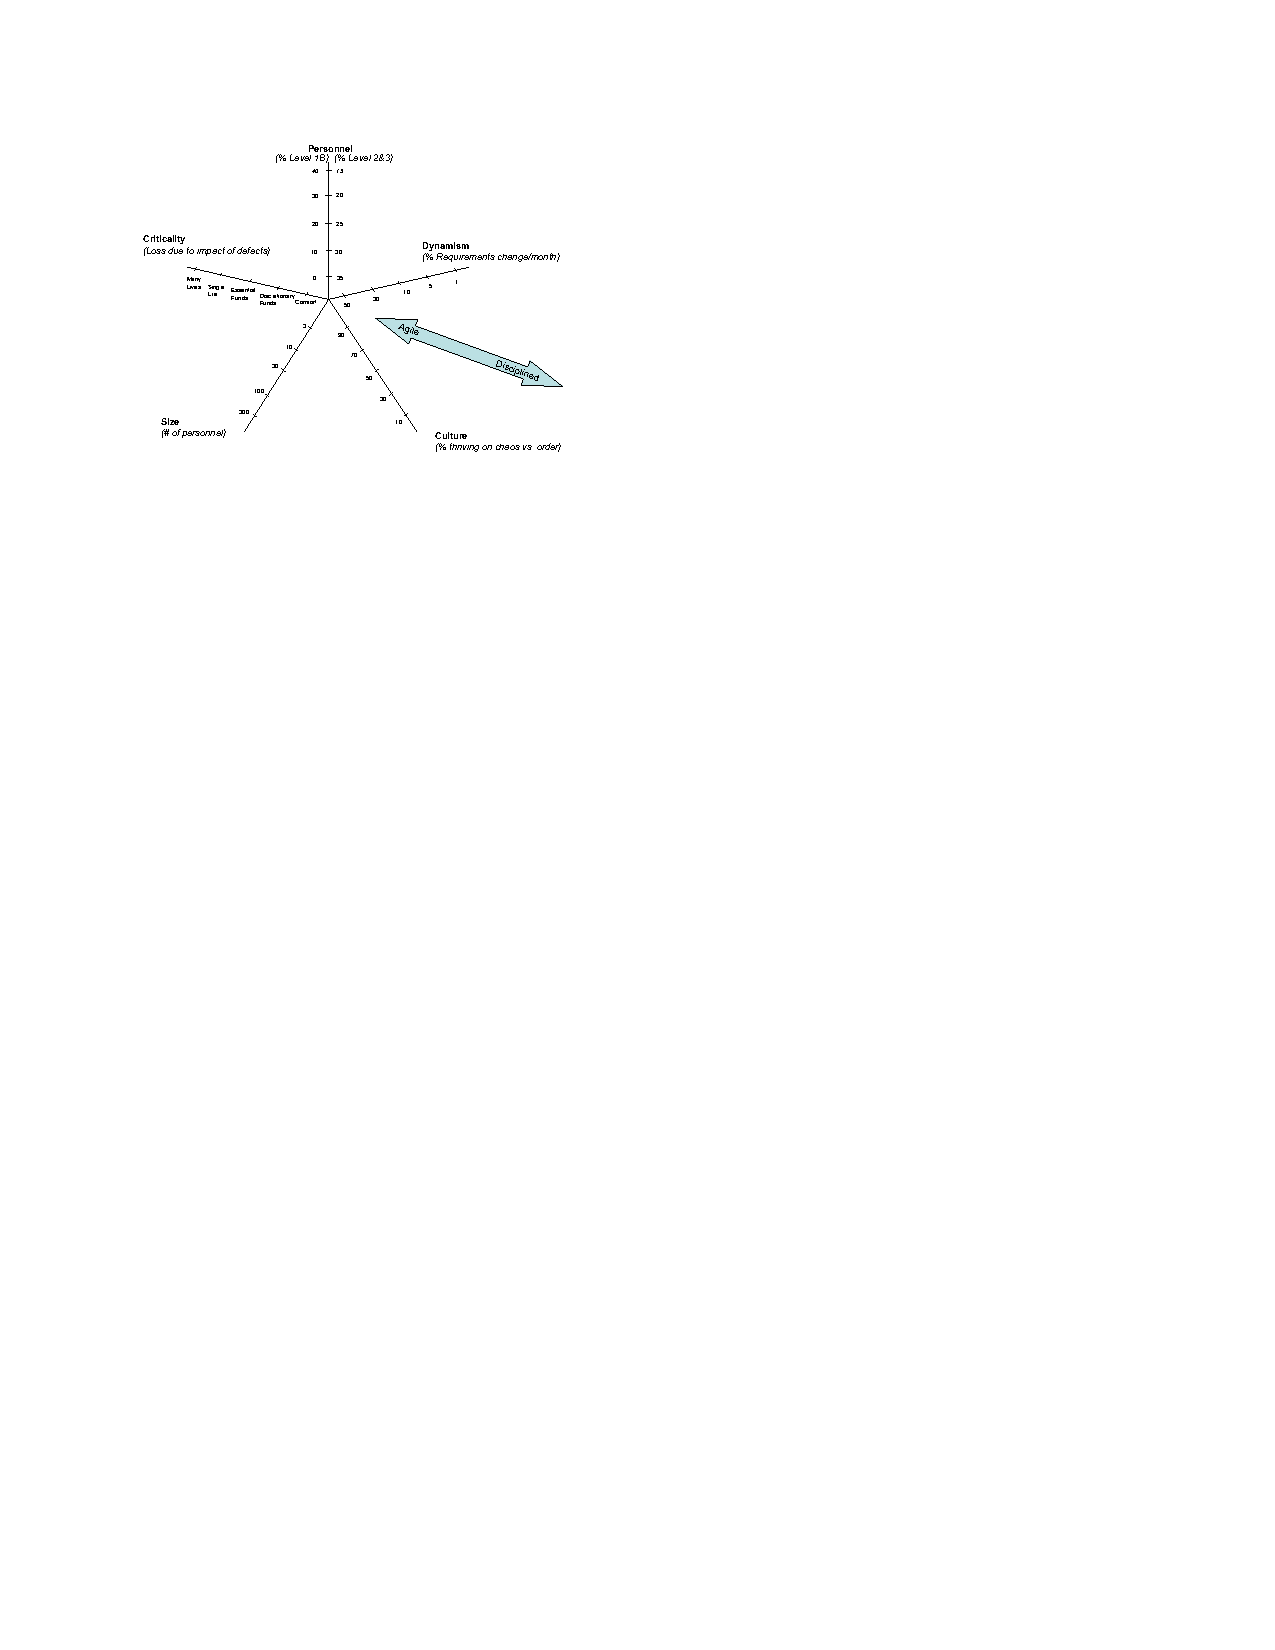
\includegraphics[scale=0.9]{include/relatedwork/fig/boehm_turner_5axes.pdf}}
{\caption{Dimensions affecting method selection} 
\label{fig:boehm_turner_5axes}}
\end{figure}

If the ratings of the five factors are close to the center, then the team is to an agile territory, in other words, the team is considered agile, otherwise it follows a discipline approach.

\subsection{Philip Taylor - Assessing Tool} 
\citet{taylor} modified the tool created by \citet{1231450} by adding a sixth axis named \textit{Client Involvement} which has the following categories:

\begin{itemize}
\item On AB - Client is on-site and an agile believer. This is the ideal when the clients are fully persuaded of the agile approach and make themselves available onsite to work with the team.
\item Off AB - Client is off-site but an agile believer. Although off-site, the client fully understands the nature of agile development and is open to frequent communication.
\item On AS - Client is on-site but is an agile skeptic. They may be on-site but they are not convinced about the agile development approach.
\item Off AS - Same as On AS except the problem is compounded by the client being off-site.
\item Off Uninvolved - Not only are the clients off-site but they want no involvement between providing the initial requirements and getting the right product delivered.
\end{itemize}

\subsection{Datta - Agility Measurement Index} %Does not measure current level of agility
\citet{datta_dissertation} presented a metric to help in deciding which agile methodology best suits a project. The metric identifies five dimensions: 
\begin{inparaenum} [a\upshape)]
\item Duration
\item Risk
\item Novelty
\item Effort
\item Interaction.
\end{inparaenum}
For each one of these dimensions the user assigns a value, then by the use of a formula the user can identify whether Waterfall, Unified Process or eXtreme Programming is more appropriate.

\subsection{Comprehensive Evaluation Framework for Agile Methodologies}
\citet{cefam} created the ``Comprehensive Evaluation Framework for Agile Methodologies" (CEFAM) in order to provide coverage to the important aspects of agile methodology. The tool consists of a hierarchy of evaluation criteria which are divided into five groups (see Figure~\ref{cefam})
\begin{inparaenum} [a\upshape)]
\item Process
\item Modeling Language
\item Agility
\item Usage
\item Cross-Context.
\end{inparaenum}
Each of these groups has a number of questions which are either answered with a numeric value, with Yes/No or any value from a proposed set. In the end, the answers are evaluated based on the following scale: Unacceptable $\leq$ 0.25; 0.25 < Low $\leq$ 0.5; 0.5 < Medium $\leq$ 0.75; 0.75 < High $\leq$ 1.0.

\begin{figure} [H]
\centerline{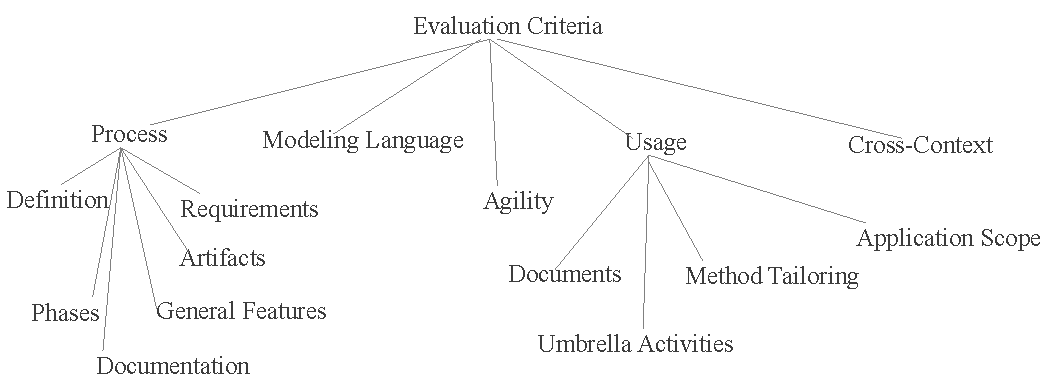
\includegraphics[scale=0.75]{include/relatedwork/fig/cefam.pdf}}
\caption{Evaluation criteria hierarchy for CEFAM} 
\label{cefam}
\end{figure}

\subsection{4-Dimensional Analytical Tool} %Does not measure current level of agility --- Part of framework
\citet{qumer2006measuring} created the 4-Dimensional Analytical Tool (4-DAT) for analysing and comparing agile methods which is a part of the of the Agile Adoption and Improvement Model (AAIM) \cite{qumerAAIM}. The objective of the tool is to provide a mechanism for assessing the degree of agility and adaptability of any agile methodology. The measurements are taken at a specific level in a process and use specific practices.

\paragraph{Dimension 1 - Method Scope Characterization}
The first dimension describes the key scope items which are considered essential for supporting the method used by a team or organisation. These have been derived from the literature review of the creators based on \citet{Beck:2004:EPE:1076267}, \citet{koch2005agile}, \citet{Palmer:2001:PGF:600044}, \citet{Highsmith:2000:ASD:323922} and provides a method comparison at a high level.


%These items are:
%\begin{inparaenum} [a\upshape)]
%\item Project Size
%\item Team Size
%\item Development Style
%\item Code Style
%\item Technology Environment
%\item Physical Environment
%\item Business Culture
%\item Abstraction Mechanism
%\end{inparaenum}

%The aforementioned elements are considered essential for supporting the method used by a team or organisation. Table~\ref{fig:dimension1} provides a description for the items.
%
%\begin{table}[H]
%\caption{4-DAT Dimension 1}
%\label{fig:dimension1}
%\centerline{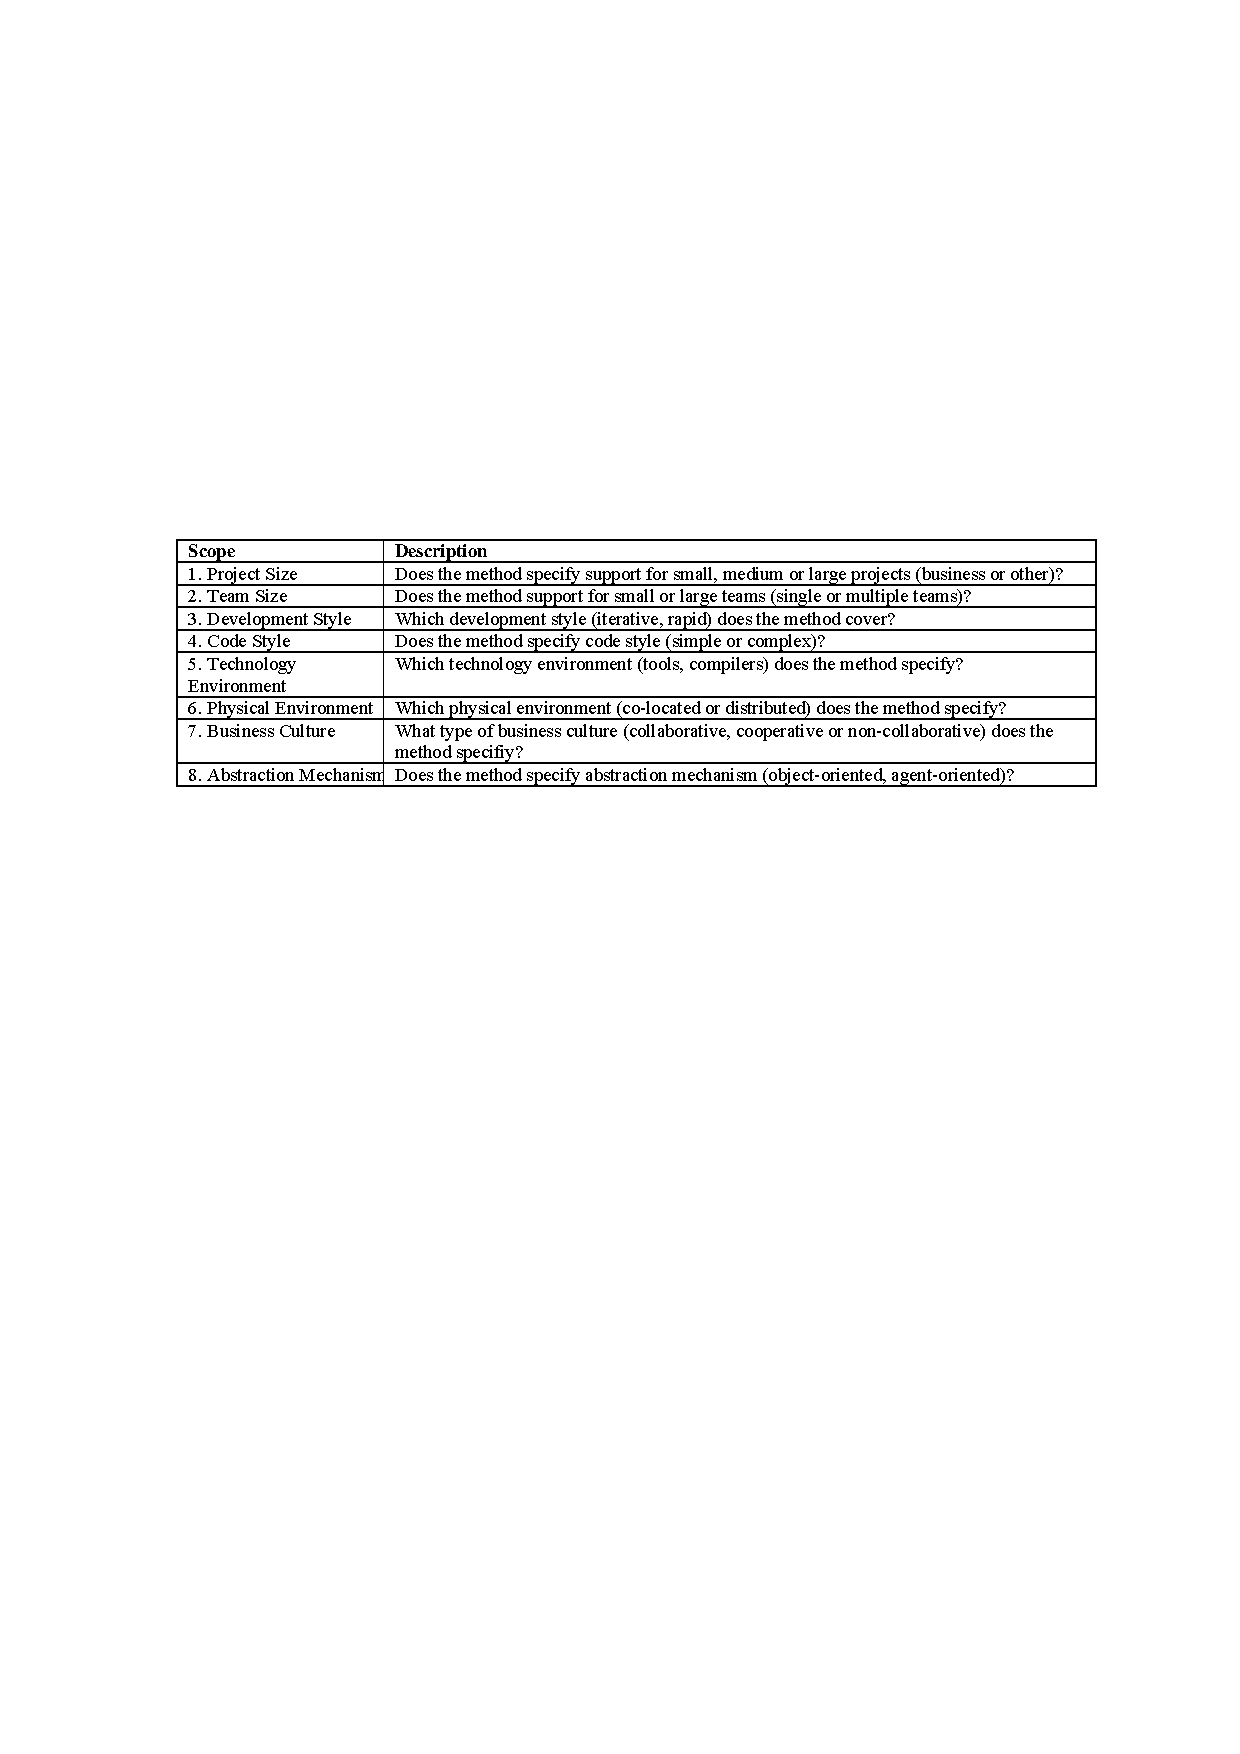
\includegraphics[scale=0.8]{include/relatedwork/fig/qumer_dimension1.pdf}}
%\end{table}

\paragraph{Dimension 2 - Agility Characterization}
The second dimension is the only quantitative dimension among the four.  It evaluates the agile methods at a process level and at a method practices level in order to check for the existence of agility.

The measurement of the degree of agility at this level is done based on five variables. %Table~\ref{fig:dimension2} provides a description for them.
%\begin{inparaenum} [a\upshape)]
%\item Flexibility
%\item Speed
%\item Leanness
%\item Learning
%\item Responsiveness
%\end{inparaenum}

These variables are used to check the existence of a method's objective at a specific level or phase. If the variable exists for a phase, then the value 1 is assigned to it, otherwise 0. \citet{qumer2006measuring} define the degree of agility (DA) as ``the fraction of the five agility variables that are encompassed and supported". They define as \textit{Object} an object at some level or lifecycle phase or as a result of the practices used. \textit{m} is the number of phases or  practices. \textit{Phase} is any of the design, planning phase or requirements engineering phase. \textit{Practice} is the practices of the agile methodology. \\ %maybe provide an example as the authors do

Formula \eqref{eq:dat_formula} how DA is calculated\\
\begin{equation} \label{eq:dat_formula} DA (Object) = (1/m) \sum m DA(Object, Phase Or Practices) \end{equation}

%\begin{table}[H]
%\caption{4-DAT Dimension 2}
%\label{fig:dimension2}
%\centerline{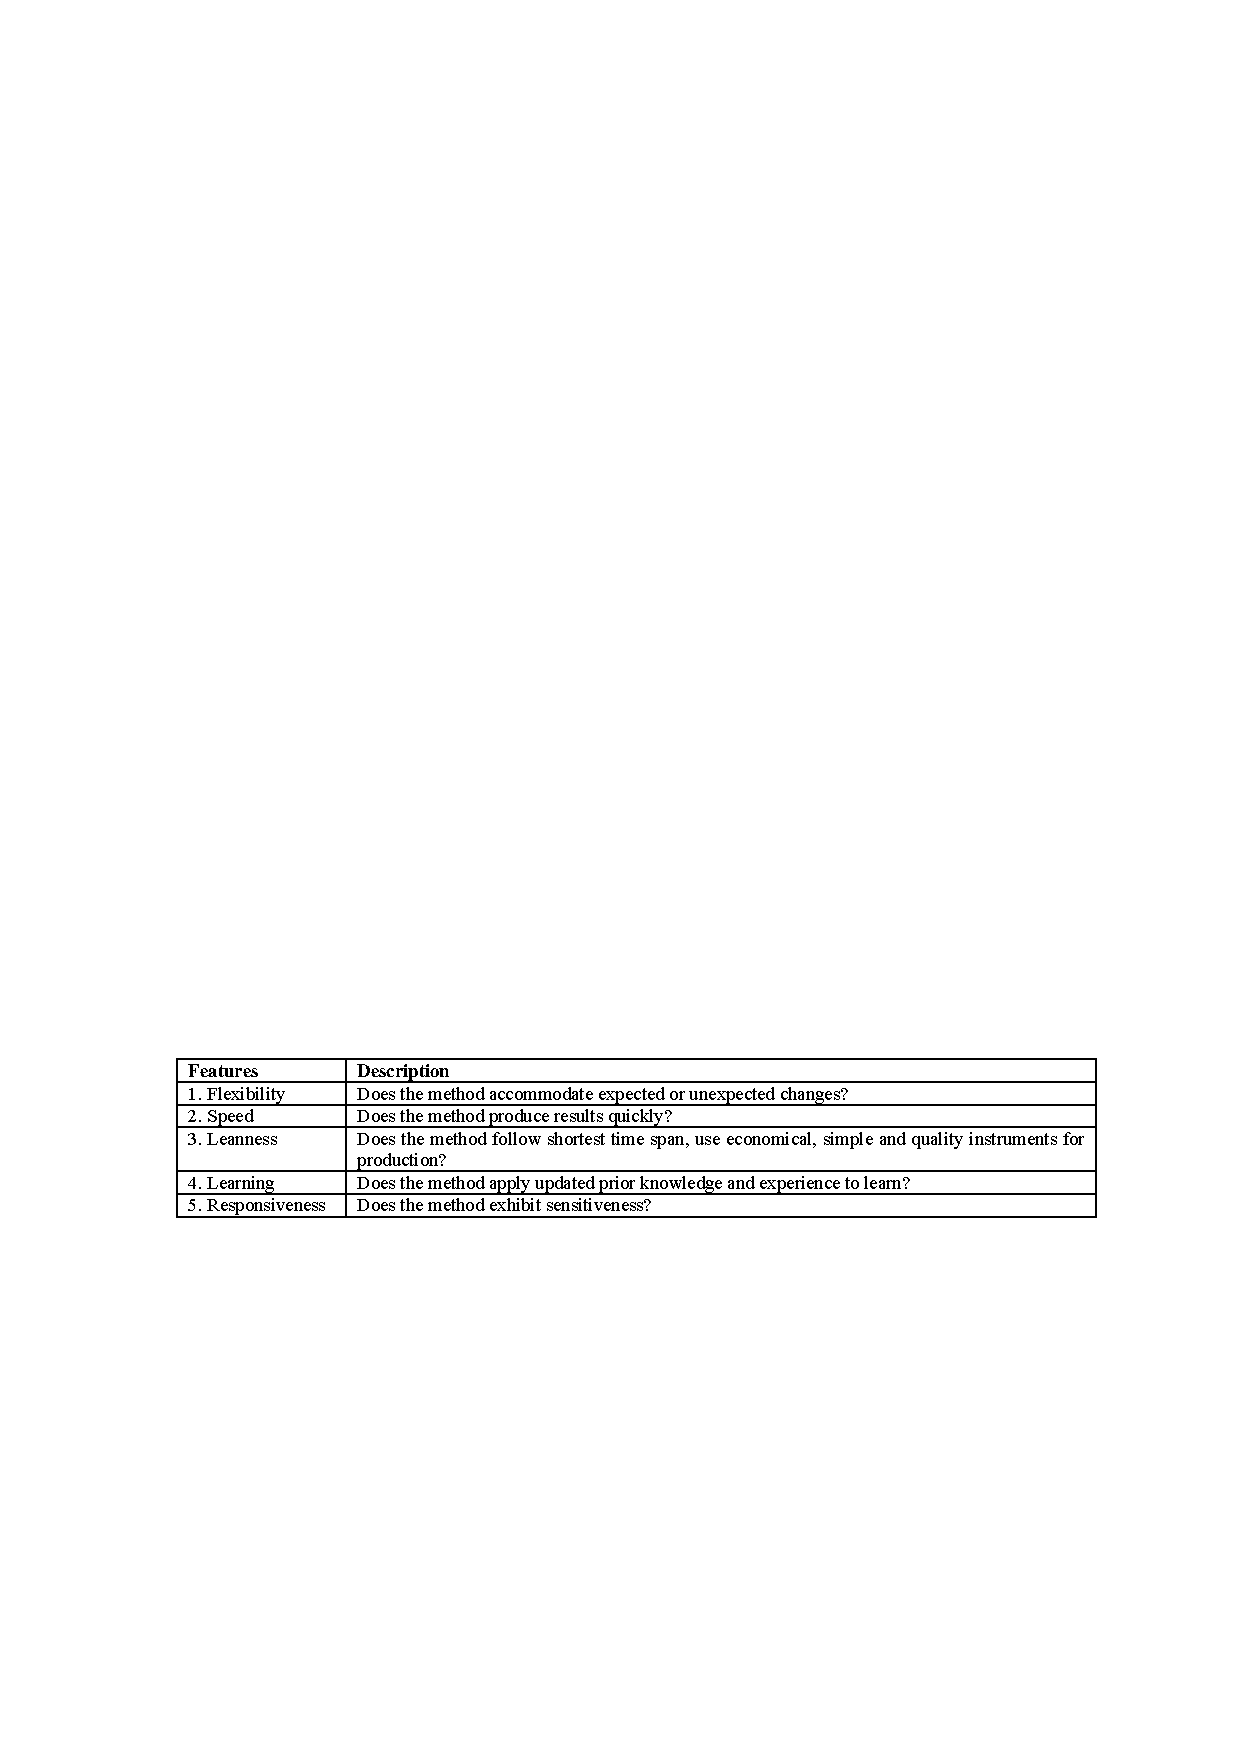
\includegraphics[scale=0.8]{include/relatedwork/fig/qumer_dimension2.pdf}}
%\end{table}

\paragraph{3 - Agile Values Characterization}
The third dimension consists of six agile values. Four of them are derived directly from the Agile Manifesto \cite{beck2001agile}, while the fifth comes from \citet{koch2005agile}. The last value is suggested by \citet{qumer2006measuring}, after having studied several agile methods. The values can be seen in Table~\ref{table:4dat_dimensions}.
%Table~\ref{fig:dimension4} shows the agile values.

%\begin{table}[H]
%\caption{4-DAT Dimension 3}
%\label{fig:dimension3}
%\centerline{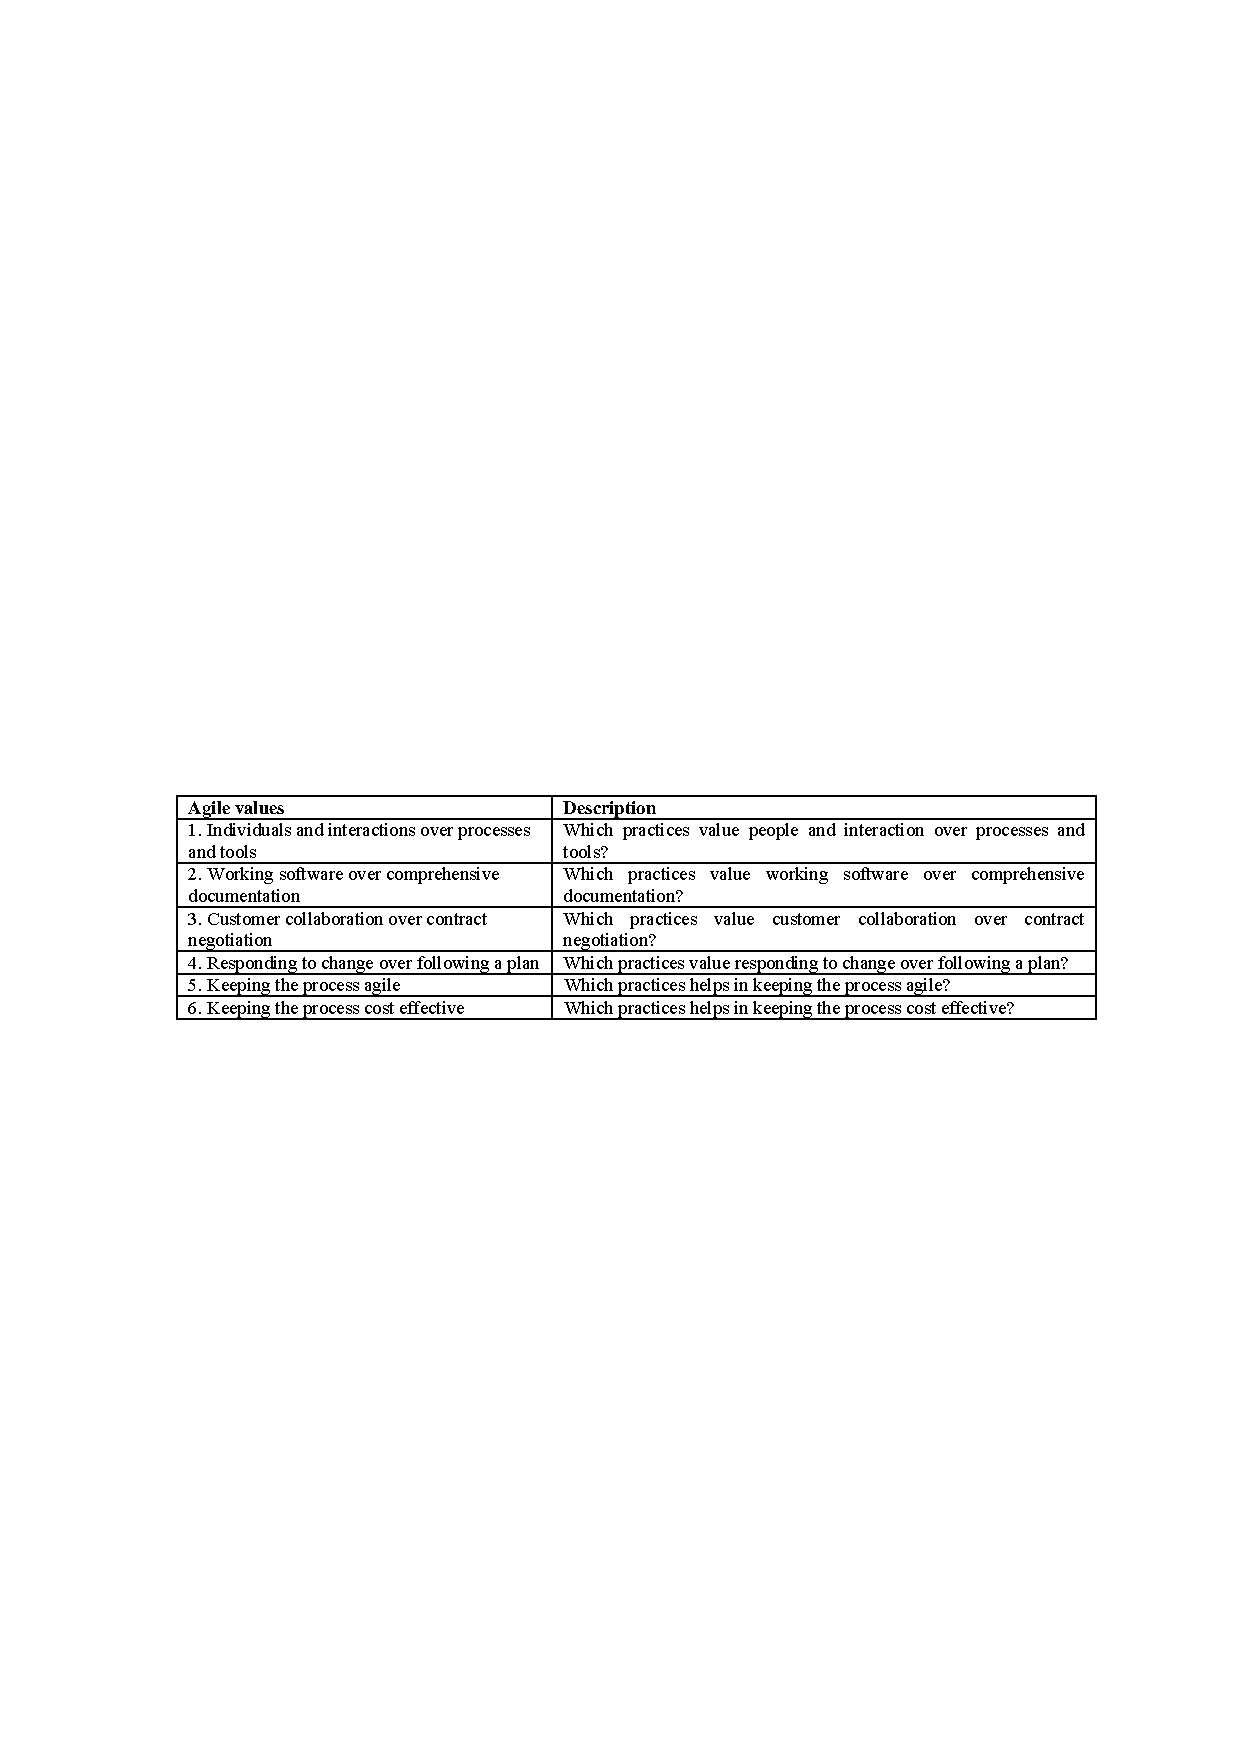
\includegraphics[scale=0.8]{include/relatedwork/fig/qumer_dimension3.pdf}}
%\end{table}

\paragraph{Dimension 4 - Software Process Characterization}
The fourth dimension examines the practices that support four processes as these are presented by \citet{qumer2006measuring}. %Table~\ref{fig:dimension4} lists these processess.

\begin{table} [H]
\caption{4-DAT Dimensions}
\label{table:4dat_dimensions}
\begin{tabular}{ | p{3cm} | p{11cm} |} \hline
	D1 - Scope & \begin{inparaenum} [a\upshape)]
		\item Project Size
		\item Team Size
		\item Development Style
		\item Code Style
		\item Technology Environment Responsiveness
		\item Physical Environment
		\item Business Culture
		\item Abstraction Mechanism
	\end{inparaenum} \\ \hline
	D2 - Features & \begin{inparaenum} [a\upshape)]
		\item Flexibility
		\item Speed
		\item Leanness
		\item Learning
		\item Responsiveness
	\end{inparaenum} \\ \hline
	D3 - Agile values & \begin{inparaenum} [a\upshape)]
		\item Individuals and interactions over processes and tools
		\item Working software over comprehensive documentation
		\item Customer collaboration over contract negotiation
		\item Responding to change over following a plan
		\item Keeping the process agile
		\item Keeping the process cost effective
	\end{inparaenum} \\ \hline
	D4 - Process & \begin{inparaenum} [a\upshape)]
		\item Development Process
		\item Project Management Process
		\item Software Configuration Control Process / Support Process
		\item Process Management Process
	\end{inparaenum}\\ 
	\hline
\end{tabular}
\end{table}

%\begin{table}[H]
%\caption{4-DAT Dimension 4}
%\label{fig:dimension4}
%\centerline{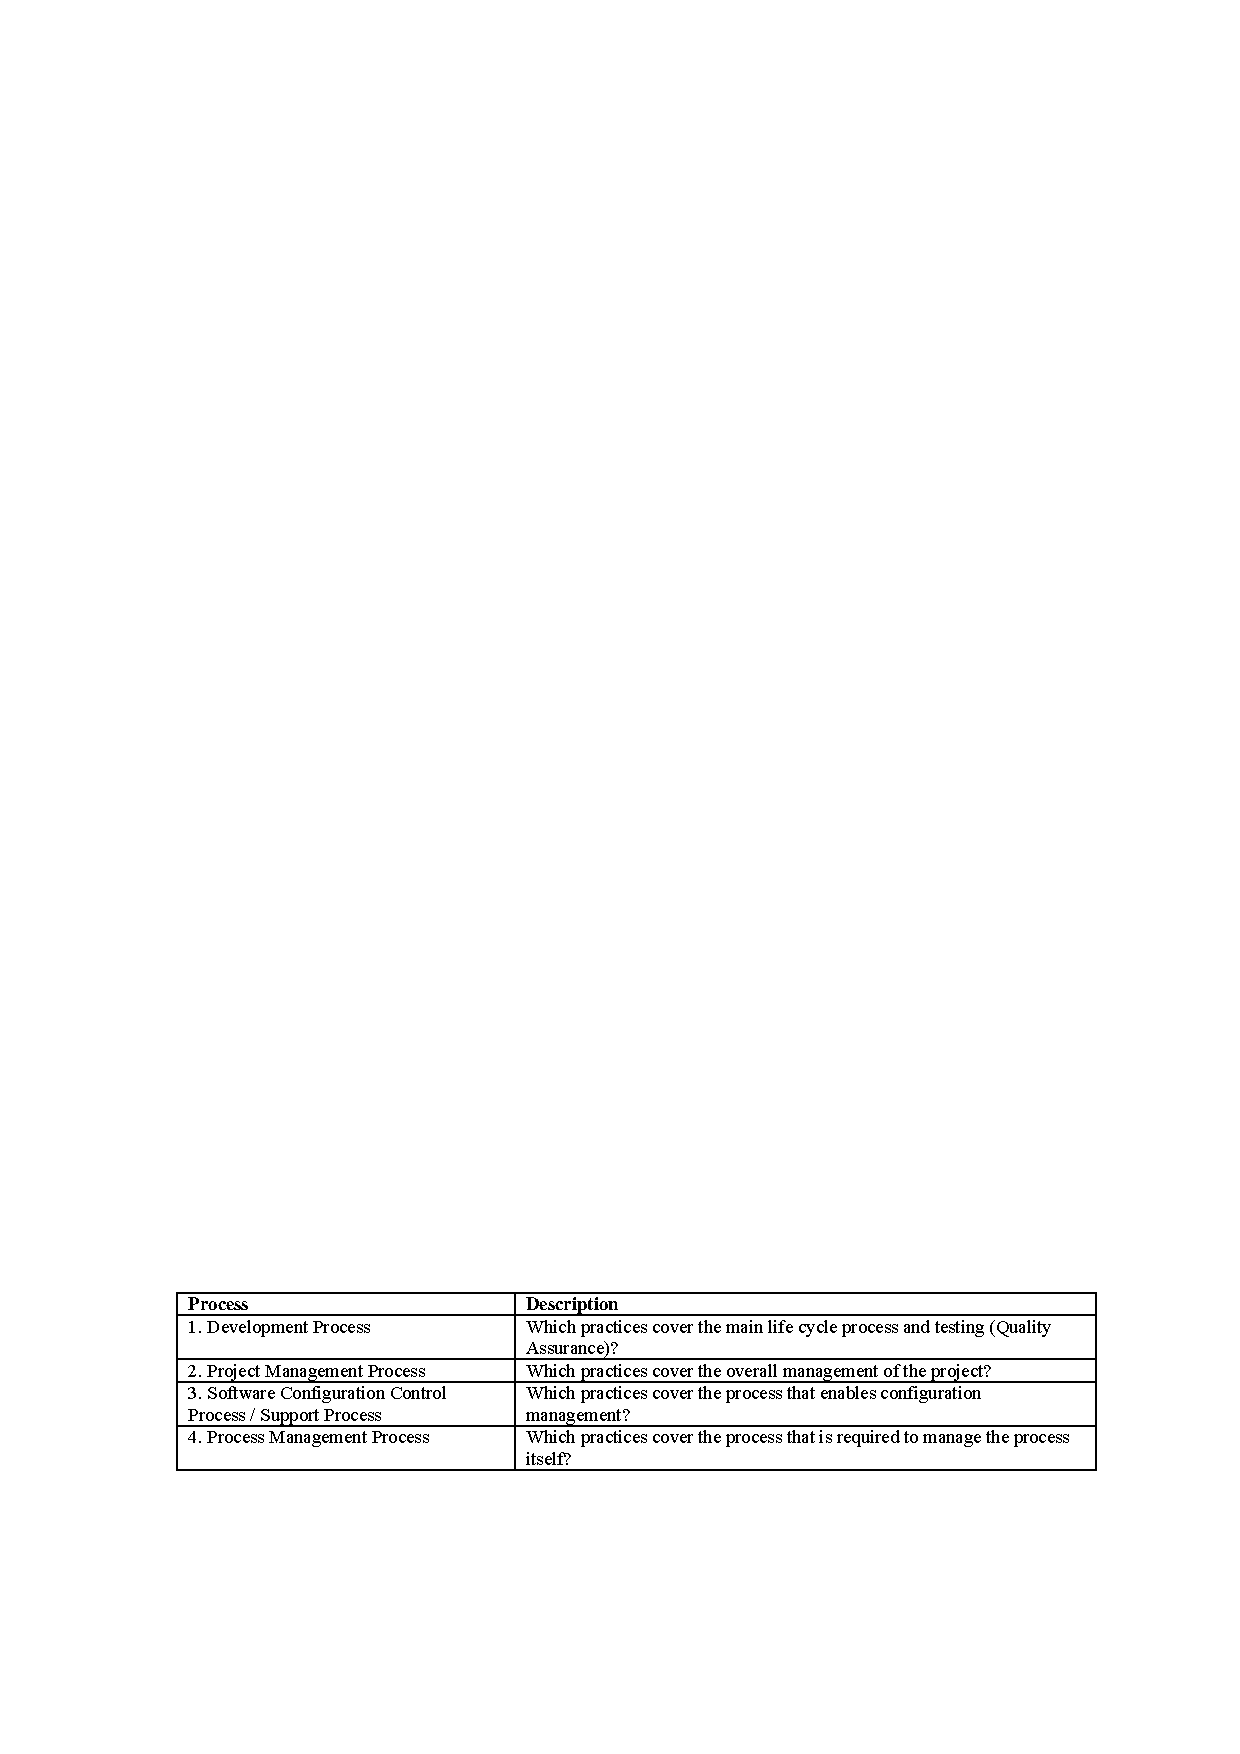
\includegraphics[scale=0.8]{include/relatedwork/fig/qumer_dimension4.pdf}}
%\end{table}

\subsection{XP Evaluation Framework} % Framework ---- Not sure for the section
\citet{williams2004toward} proposed a framework named the ``XP Evaluation Framework" (XP-EF) for assessing the XP practices which have been adopted by an organisation. The framework consists of three parts
\begin{itemize}
	\item XP Context Factors (XP-CF) - Record important contextual information. The factors can be team size, project size, staff experience
	\item XP Adherence Metrics (XP-AM) - Express in a precise way the practices utilized by a team
	\item XP Outcome Measures (XP-OM) - A Means to assess the outcomes of a project using full or partial XP practices
\end{itemize}



\section{Agility of Software Development Teams}

\subsection{Team Agility Assessment} %write more %Measures current level of agility
%Mention it is Scrum oriented
\citet{Leffingwell} created a model for assessing a team's agility by
 taking six aspects into account:
\begin{inparaenum} [a\upshape)]
\item Product Ownership
\item Release Planning and Tracking
\item Iteration Planning and Tracking
\item Team
\item Testing Practices
\item Development Practices/Infrastructure.
\end{inparaenum}

Each of these aspects is followed by a number of questions rated on a six-point Likert scale and the results are represented in a radar chart.

\subsection{Comparative Agility} %Current level of agility
\citet{comparative_agility} created the Comparative Agility (CA) assessment tool which does not assess the agility of an organisation by providing an absolute value, but it rather provides a value in comparison to other organisations/companies \cite{comparative_agility_web}. The idea behind CA is that the organisations try to be more agile than their competitors because they believe that this will have more benefits for them. Until 2010, more than 1200 respondents supported that idea by answering the tool's online survey. The CA assessment tool consists of the following seven dimensions
\begin{inparaenum} [a\upshape)]
	\item Teamwork
	\item Requirements
	\item Planning
	\item Technical Practices
	\item Quality
	\item Culture
	\item Knowledge-Creating,
\end{inparaenum}
which are made up of three to six characteristics. Each characteristic has four statements and each one of them represents an agile practice. The answers to every statement are measured on a five-point Likert scale.

\subsection{Escobar - Vasquez Model for Assessing Agility} %Measures current level of agility

\citet{6427226} created their own agility assessment model which consists of four stages. For the first three they use the models and tools proposed by other researchers they found in literature.
\begin{itemize}
\item Agile Project Management Assessment - proposed by \citet{qumer2006measuring}
\item Project Agility Assessment - proposed by \citet{taylor}
\item Workteam Agility Assessment - proposed by \citet{Leffingwell}
\item Agile Workspace Coverage
\end{itemize}

For collecting the data on the measurements, they used surveys based on the tools of each stage, while in the last one they use their own survey. The data are then depicted in a four axis radar chart in order to provide a view of the company's agility. In Figure~\ref{escobar_model}, one can see the model with a short description about which tool should be used at each level for each stage.

\begin{figure} [H]
\centerline{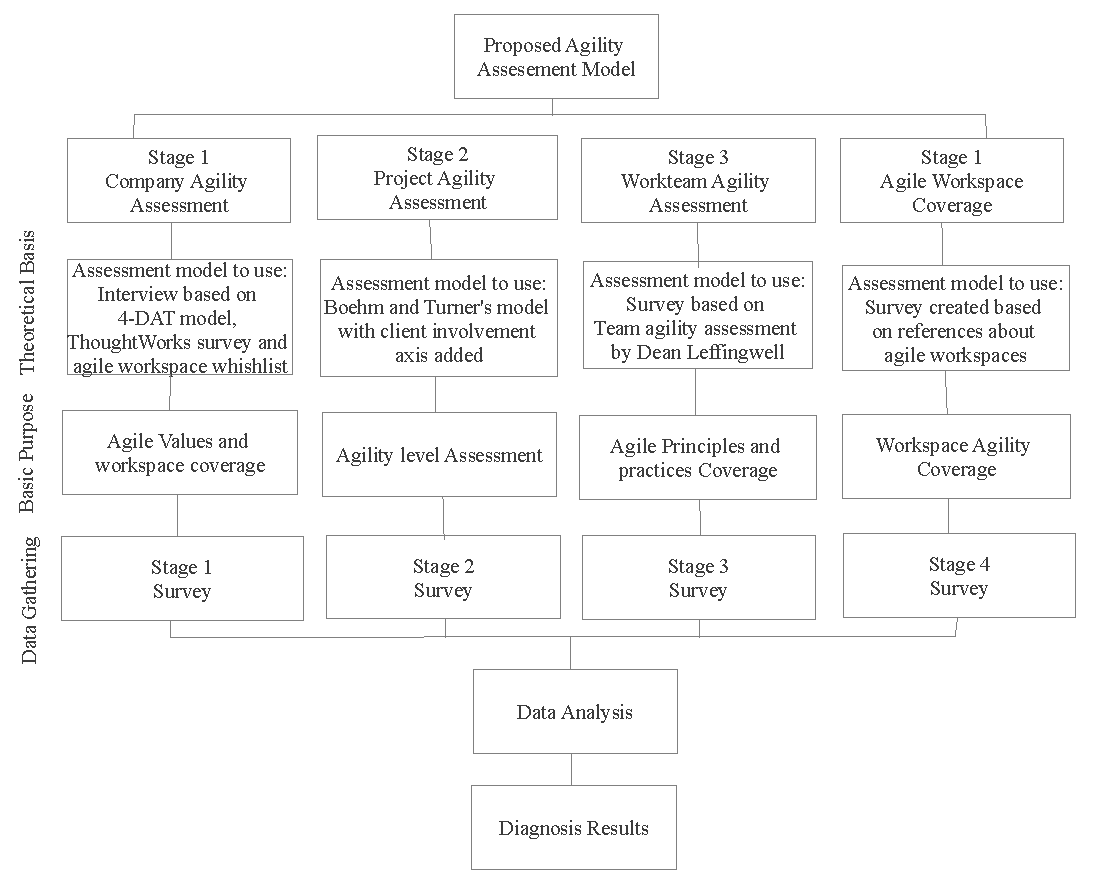
\includegraphics[scale=0.75]{include/relatedwork/fig/escobar_model.pdf}}
\caption{Escobar - Vasquez model for assessing agility} 
\label{escobar_model}
\end{figure}

\subsection{Entropy Analysis}
\citet{entropy} measure the agility based on the rate of entropy change over the time of a system's development. If the rate is high, then the process is of high agility as well. Each feature is considered to be an entity and the change logs of the entities are analyzed. They define as $P_i(t)$  the probability of an entity \textit{i} to be associated with the change logs at a time \textit{t}. Then, by using formula~\eqref{eq:entropy_analysis_formula}, they make the calculation for the agility measure \textit{AM(t)} for that specific time.

\begin{equation} \label{eq:entropy_analysis_formula} AM(t) = - \sum_{i=1}^{n} P_i'(t) (log_2 P_i(t) + 1.44) \end{equation} 

\subsection{Validation Model to Measure the Agility}
\citet{validation_model} measure agility by creating a validation model, since according to them, only validation can confirm the quality of a product. In this model any candidate item for validation enters an ``identified planning state" at planning time. Afterwards, these items change to the ``unvalidated inventory state" when the items start to be generated. Finally, validation of the deliverable items changes the state to the ``validated product state" (see Figure~\ref{validation_model}). Then, based on the formula~\eqref{eq:validation_model_formula}, one can get the result. \textit{A} is the agility of a project/organisation, \textit{V'} is the number of software items in the ``validated product state" and \textit{U'} is the average number of software items in which intermediate deliverables are in the ``unvalidated inventory state".

\begin{equation} \label{eq:validation_model_formula}  A = V'/U' \end{equation}

\subsection{Perceptive Agile Measurement}
\citet{pam} created a survey for measuring agility from a social-psychological perspective, covering eight agile practices which they named as scales. These scales are an attempt to establish a representative set of agile practices commonly used in the field

\begin{inparaenum} [a\upshape)]
\item Iteration Planning
\item Iterative Development
\item Continuous Integration and Testing
\item Co-Location
\item Stand-up Meetings
\item Customer Access
\item Customer Acceptance Tests
\item Retrospectives.
\end{inparaenum} The survey is on a seven-point Likert scale, except from the \textit{Co-Location} which is on a five-point scale.

\begin{figure} [H]
\centerline{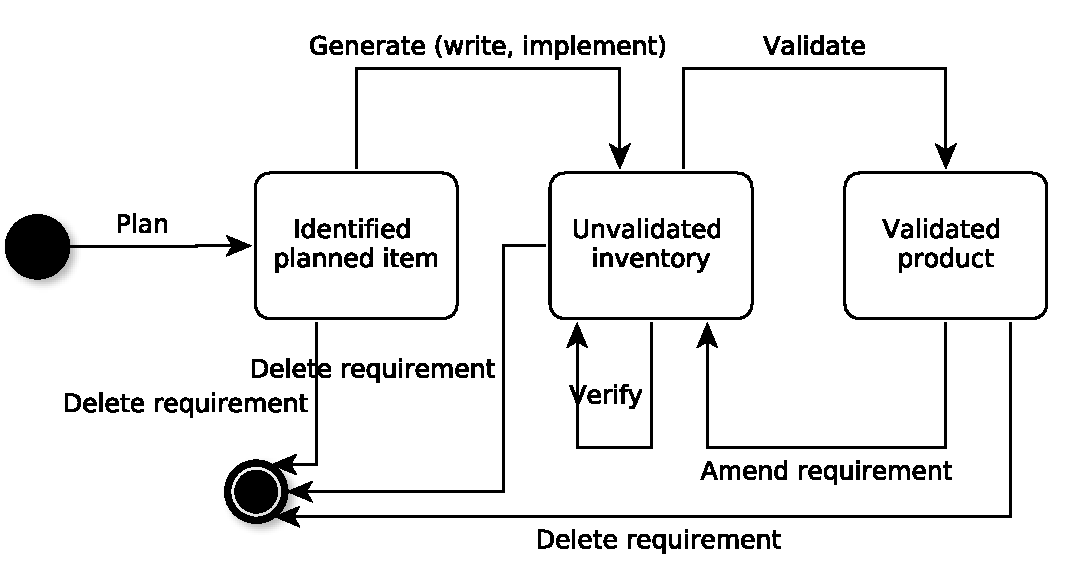
\includegraphics[scale=0.6]{include/relatedwork/fig/validation_model.pdf}}
\caption{Validation Model to Measure the Agility} 
\label{validation_model}
\end{figure}

\subsection{AHP - ANFIS Framework} %Framework
\citet{poonacha} created a tool for measuring agility by identifying 17 parameters grouped in four parameter groups, as can be seen in Table~\ref{anfis_framework}. While the last group is an indicator of performance, the first three groups mitigate the risks of supply, operation and demand uncertainties respectively. Each parameter is given as a question and the answers are fed in the Adaptive Network based on Fuzzy Inference Systems (ANFIS). Due to the complexity of the ANFIS model, an Analytical Hierarchical Process (AHP) is mandatory to be applied at the parameter level in order to compute the values for the parameter groups and then employee ANFIS at the parameter group level.

\begin{table} [H]
\begin{tabular}{| p{3cm} | p{12cm}|}
    \hline
     \textbf{Group} & \textbf{Parameters} \\ \hline
     People  &  \begin{inparaenum} [a\upshape)] \item Attrition \item Functional Flexibility \item Training and Knowlegde \item Decentralized Decision Making \item Bench Strength \end{inparaenum} \\ \hline
     Processes  & \begin{inparaenum} [a\upshape)] \item Pair Programming and Parallel Testing \item Iterative Development \item Degree of modularity \item Requirement Capture Process \item Reusability \item Continuous Improvement
     \end{inparaenum} \\ \hline
    Customer Involvment & \begin{inparaenum} [a\upshape)] \item Customer Involvement in Design \item Team Across Company Borders \item Customer Training Period \end{inparaenum} \\ \hline
     Cost and Quality  & \begin{inparaenum} [a\upshape)] \item Cost of Requirement change \item Projects dropped due to incapacity \item Software Quality \end{inparaenum} \\ \hline
  \end{tabular}
\caption{AHP - ANFIS Framework parameters}
\label{anfis_framework}
\end{table}

\subsection{42-Point Test}
\citet{42points} created a simple 42-question survey based on a similar one from Nokia \cite{nokia}, in order to allow to Scrum/XP teams to easily see to what extent they follow various agile practices.

\subsection{Sidky Agile Measurement Index}
\citet{sidky_dissertation} created the Sidky Agile Measurement Index (SAMI) in order to measure agility as a part of the ``Agile Adoption Framework". SAMI is a scale used by an agile coach to identify the potential of a project or organisation \cite{sidky}, which consists of five agile levels and five agile principles. It derives from the agile manifesto \cite{beck2001agile} and forms a $5\times 5$ matrix. Agile practices have been assigned to most of the cells of this matrix. The assessment of agility takes place at each level by measuring the practices adopted by a team. Before moving to the next level, the team needs to fulfill all the practices of the current one.

\begin{minipage}[t]{0.35\linewidth}
    \textbf{Agile Levels}
    \begin{itemize}
    \item{Level 1 - Collaborative}
    \item{Level 2 - Evolutionary}
    \item{Level 3 - Effective}
    \item{Level 4 - Adaptive}
    \item{Level 5 - Ambient}
    \end{itemize}
    \end{minipage}
    \begin{minipage}[t]{0.6\linewidth}
    \textbf{Agile Principles}
    \begin{itemize}
    \item{Embrace Change to Deliver Customer Value}
    \item{Plan and Deliver Software Frequently}
    \item{Human Centric}
    \item{Technical Excellence}
    \item{Customer Collaboration}
    \end{itemize}
\end{minipage}

\subsection{Thoughtworks} %Measures current level of agility
Thoughtworks \cite{thoughtworks} is a worldwide consulting company. They have developed an online survey for assessing agility based on 20 multiple choice questions. The questions cover the areas of 
\begin{inparaenum} [a\upshape)]
	\item Requirements Analysis
	\item Business Responsiveness
	\item Collaboration and Communication
	\item Project Management
	\item Governance.
\end{inparaenum}
People can answer to the survey online and they will get a report evaluating at which level their team or company is. The survey gained a lot of fame due to Martin Fowler, one of the creators of the agile manifesto working at the company.

\subsection{Objectives Principles Strategies Framework}
\label{subsec:ops}
\citet{sventha_dissertation} created the Objectives, Principles and Stategies (\ac{OPS}) Framework in order to assess the ``goodness" of an agile methodology. It is an evolution of the work done by \citet{2604} and \citet{sidky_dissertation}. The focus of this tool is mainly on eXtreme Programming, Feature Driven Development, Lean, Crystal and any tailored instances of them.

In order to achieve this, the framework examines the methodology based on 3 aspects:
\begin{itemize}
\item Adequacy - Sufficiency of the method with respect to meeting its stated objectives.
\item Capability - Ability of an organisation to provide an environment supporting the implementation of its adopted method. Such ability is reflected in the characteristics of an organisation's people, process
and project.
\item Effectiveness - Producing the intended or expected results. The existence of necessary process, artifacts and product characteristics indicate levels of effectiveness.
\end{itemize}

%add figure 3.9

The \ac{OPS} framework identifies 
\begin{inparaenum} [a\upshape)]
\item objectives of the agile philosophy
\item principles that support the objectives
\item strategies that implement the principles
\item linkages that relate objectives to
principles, and principles to strategies
\item indicators for assessing the extent to which an organisation supports the implementation and effectiveness of those strategies.
\end{inparaenum}

%The \ac{OPS} Framework identifies 
%\begin{itemize}
%\item Objectives of the agile philosophy - ``something aimed at or striven for" as defined by \citet{2604}
%\item Principles - what rules a process in order to achieve an objective according to \citet{2604}
%\item Strategies - the implementations of the principles (i.e. they are the means for achieving the principles)
%\item Linkages - the connectors between 
%\begin{inparaenum} [a\upshape)]
%\item the objectives and principles, 
%\item the principles and the strategies. 
%\end{inparaenum} 
%The linkages show the path in order to asses the adequacy, capability and effectiveness of the method used.
%\item Indicators for assessing the extent to which an organisation supports the implementation and effectiveness of those strategies - In order to measure the capability and the effectiveness the strategies use properties which contain a number of questions. These properties differ for the capability and the effectiveness. Indicator is named the combination of a strategy with a property. They are directly measurable and are tailored to assess the strategies
%\end{itemize}

In total 5 objectives, 9 principles, 17 strategies, 54 linkages and 80 indicators are identified. For more information, one can view  Figure~\ref{objectives_principles_strategies}.

\begin{figure} [H]
\centerline{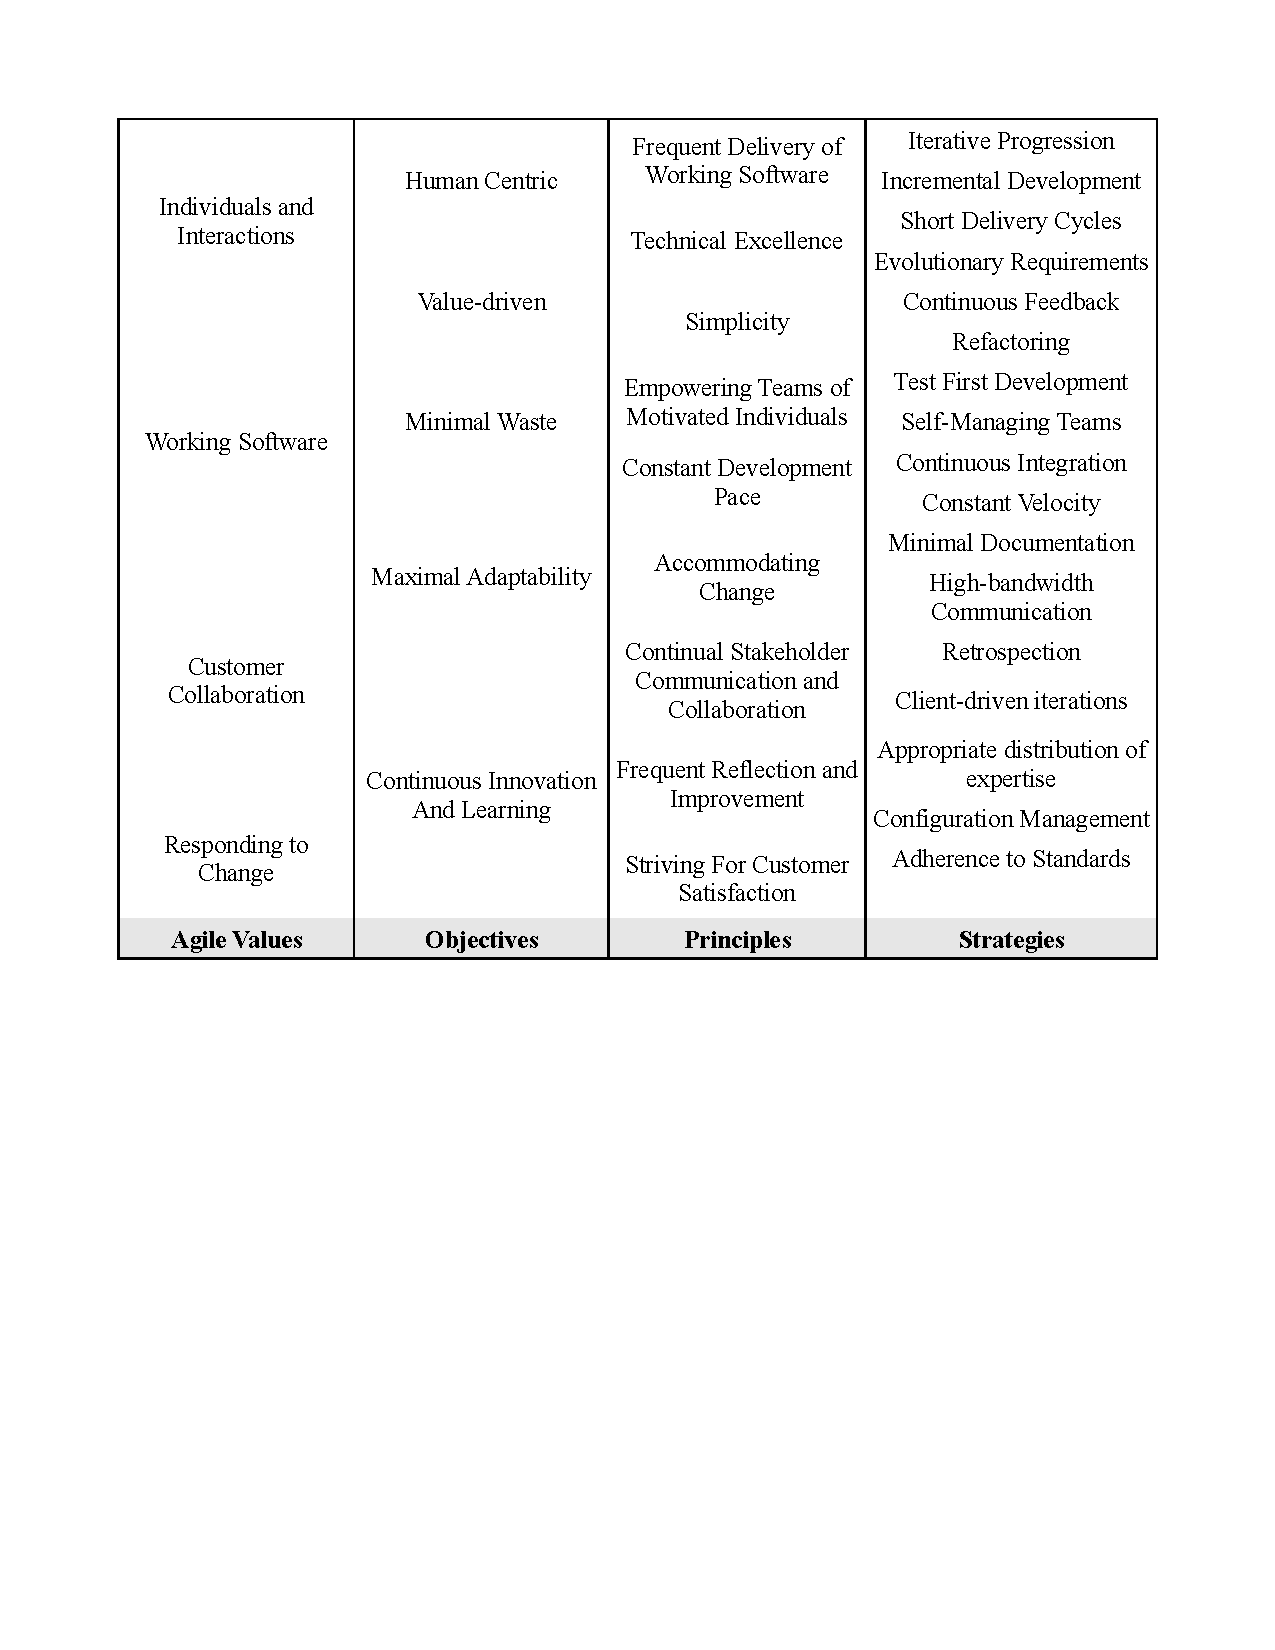
\includegraphics[scale=0.75]{include/relatedwork/fig/ops.pdf}}
\caption{Objectives, Principles, and Strategies identified by the \ac{OPS} Framework} 
\label{objectives_principles_strategies}
\end{figure} 

%The \ac{OPS} Framework works on a top down traversal for assessing the adequacy. One should identify the objectives followed by the method and based on the linkages move to the principles and then to strategies. On the other hand for assessing the capability and effectiveness the tool works on a bottom up traversal. Based on the strategies identified during the adequacy analysis one should answer the a set of questions for the capability and to another set of questions for the effectiveness. Then the measurements are propagated to the upper levels through the linkages. For a better understanding one can see Figure~\ref{ops_core}.
%
%\begin{figure} [H]
%\centerline{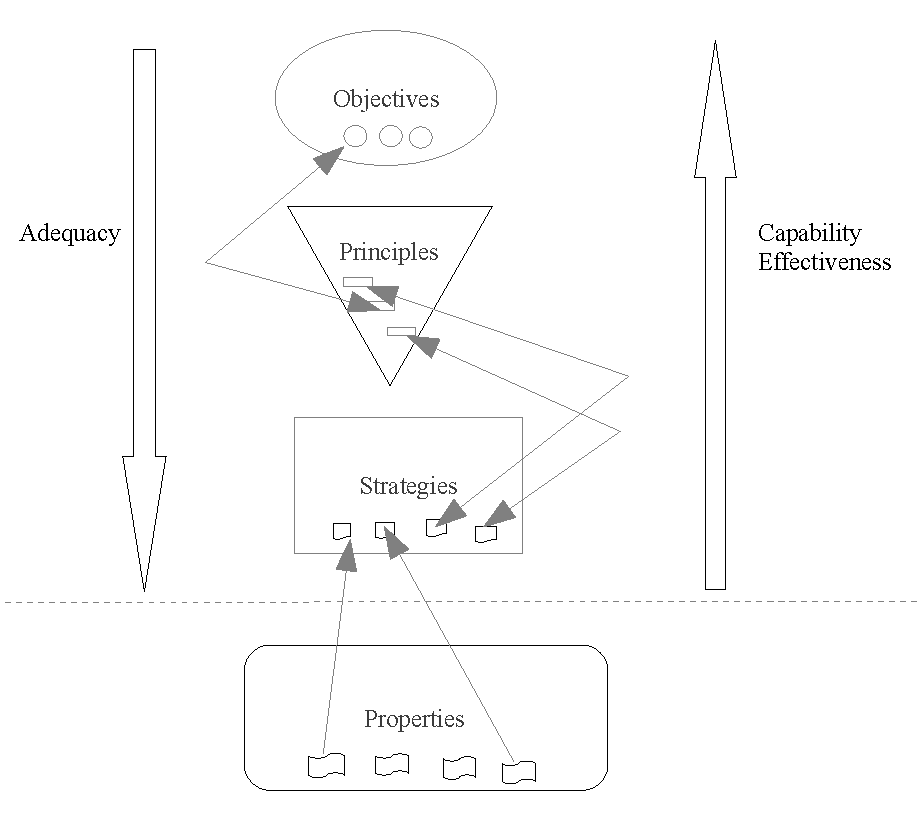
\includegraphics[scale=0.75]{include/relatedwork/fig/ops_core.pdf}}
%\caption{OPS Framework} 
%\label{ops_core}
%\end{figure} 



\section{Selecting tools}
The tools selected for the case study that follows in the next chapter are Perceptive Agile Measurement (PAM), Team Agility Assessment (TAA) and Objectives Principles Strategies (OPS). All three of them originate from either industry (\ac{TAA}) or academia (\ac{OPS}) or both (\ac{PAM}). \ac{PAM} has been used in a case study in the past with a large sample. The tool was created with participations from development teams from all over the world. \ac{TAA} is used by companies and has gained a lot of acclaim during the last years by practitioners. \ac{OPS} Framework is a fairly new and promising since it covers more agile practices than any other tool.


\section{Chapter Summary}
In this chapter were presented the most common tools found in literature for measuring agility and the reasons for selecting the ones for the case study. In the next chapter follows the case study performed in order to see how \ac{PAM}, \ac{TAA} and \ac{OPS} correlate and how complete they are among them in what they do.